\documentclass{article}

\usepackage[preprint]{neurips}

\makeatletter
\renewcommand{\@notice}{}
\makeatother

\usepackage[utf8]{inputenc}
\usepackage[T1]{fontenc}
\usepackage{amsmath}
\usepackage{amssymb}
\usepackage{booktabs}
\usepackage{graphicx}
\usepackage{adjustbox}
\usepackage{caption}
\usepackage{subcaption}
\usepackage{float}
\usepackage{placeins}
\usepackage{xcolor}
\usepackage{hyperref}
\usepackage{url}

\hypersetup{
  colorlinks=true,
  linkcolor=blue,
  citecolor=blue,
  urlcolor=blue
}

\raggedbottom
\setlength{\textfloatsep}{7pt plus 2pt minus 2pt}
\setlength{\intextsep}{7pt plus 2pt minus 2pt}
\setlength{\floatsep}{6pt plus 2pt minus 2pt}
\renewcommand{\topfraction}{0.97}
\renewcommand{\bottomfraction}{0.90}
\renewcommand{\textfraction}{0.03}
\renewcommand{\floatpagefraction}{0.88}
\setcounter{topnumber}{5}
\setcounter{bottomnumber}{4}
\setcounter{totalnumber}{9}
\captionsetup{font=small,skip=3pt}

\newcommand{\msq}{\ensuremath{\mathrm{m}/\mathrm{s}^{2}}}
\newcommand{\pct}{\%}

\title{Assignment 1 Report: Structured Time Series Forecasting with Attention and Autoformer}

\author{
  Daniyal Hussain Shah
}

\begin{document}

\maketitle

\begin{abstract}
This report studies two forecasting settings that share the same main question: how much does a suitable temporal inductive bias help compared with a more flexible model? Task 1 uses a controlled four-station vibration process. It compares fixed linear mappings, context-dependent Attention, moving-average decomposition, and delay-based mixing. Period-routed ridge gives the best deployment result because the simulated operating pace is directly available through a reliable period estimate. Among the neural designs, the Autoformer-inspired combination of decomposition and delay mixing gives the lowest validation error. Task 2 applies a from-scratch Autoformer to an anonymized, heavy-tailed series and forecasts 168 unseen observations. A chronological validation study selects moving-average width 13. A three-seed ablation shows that the ten optional external variables reduce mean validation RMSE from 88.31 to 62.19. The final model contains 42,561 trainable parameters, is trained for three epochs on all observed target values, and obtains 84.57 RMSE on the hidden leaderboard continuation. Code, executed notebooks, configurations, and machine-readable results are available at \url{https://github.com/syeddaniyalg/cs434-pa1}.
\end{abstract}

\section{Introduction}

Time-series forecasting depends on what information a model is encouraged to preserve. A general Attention layer can build a different mixing rule for every context, but it must learn periodic and slow-moving structure from data. A model with a stronger temporal assumption can separate trend from repeated variation or organize relationships by delay. These choices can improve accuracy, but they can also be unnecessary when a simple and correct physical variable is already known.

This report examines that trade-off in two tasks. Task 1 is a controlled forecasting study with known operating regimes and an unseen station. The task begins with fixed ridge mappings, introduces context-dependent Attention, then tests moving-average decomposition and temporal-delay mixing. Task 2 uses a real, anonymized target series with optional external variables. It requires a full Autoformer, a chronological validation protocol, multi-seed comparisons, and a 168-step final forecast. The Autoformer mechanisms used in both tasks follow the decomposition and auto-correlation ideas of \citet{wu2021autoformer}.

The report is organized around the decisions made in each task. Every model comparison names its population and split. Task 1 reports physical-unit errors on the supplied validation and final-test regions. Task 2 reports RMSE, MAE, and sMAPE on 26 chronological validation blocks. Figures are used to show the signal behavior behind the numerical results, while tables collect the values used for model selection.

\section{Experimental Setup}
\label{sec:setup}

\subsection{Task 1: heterogeneous vibration sensors}

The simulated production line contains four stations sampled at 20 Hz. Products A, B, and C use actual cycle lengths in the ranges 14--18, 21--27, and 28--36 samples. Each reading combines a slow 240-sample drift, a repeating station-specific vibration, and noise. A model receives a context of $L=96$ samples and predicts $H=48$ samples. Windows never cross an operating-regime boundary.

Stations 1--3 form the established population. Their samples 0--9600 are used for fitting, 9600--12480 for validation, and 12480--15360 for final testing. Station 4 is excluded from model fitting and preprocessing-statistic estimation. It still provides its own context at prediction time and therefore measures transfer to a held-out sensor. Each context is anchored at its last observed value and scaled using one statistic fitted only from established-station training data. All reported errors are converted back to physical units.

The neural comparisons use model seed 0 and the full experiment preset. The four neural variants share width, depth, data order, optimizer schedule, and checkpoint policy. They differ only in whether the input is raw or decomposed and whether the mixer is Attention or delay based. Parameter count and fit time are reported because these switches do not have identical cost.

\subsection{Task 2: anonymized long-horizon forecasting}

The observed target contains 43,656 uniformly spaced values. Its mean is 98.17, standard deviation is 90.83, and range is 0 to 994. The distribution is heavy-tailed and contains sharp level changes. The last 4,368 observed values are reserved for validation, leaving 39,288 values for training. Validation uses 26 non-overlapping forecast origins spaced by the 168-step horizon. This split is chronological, so every validation target occurs after the fitting region.

The target is standardized using the training-region mean and standard deviation. Of the ten external variables, the first six continuous variables are standardized using training-region statistics, while the four binary indicators remain unchanged. The external file covers both history and the future forecast horizon. Training windows have 672 input steps, 168 decoder label steps, and 168 target steps. Origins use stride 1, producing 38,449 training windows. Negative predictions are clipped to zero because the measured quantity is non-negative.

All reported Task 2 experiments use Adam with learning rate $10^{-3}$, batch size 64, gradient clipping at 1.0, and a three-epoch budget. Preliminary trials with five-epoch and 50-epoch budgets showed that the model made most of its useful progress within approximately three epochs. Three epochs were therefore adopted as the standard schedule for the controlled comparisons and final fit. Each validation run keeps the checkpoint with the lowest physical-unit RMSE. Width selection uses seeds 0 and 1. The external-data ablation uses matched seeds 0, 1, and 2. The final selected configuration is refitted on all observed target values.

\begin{figure}[htbp]
\centering
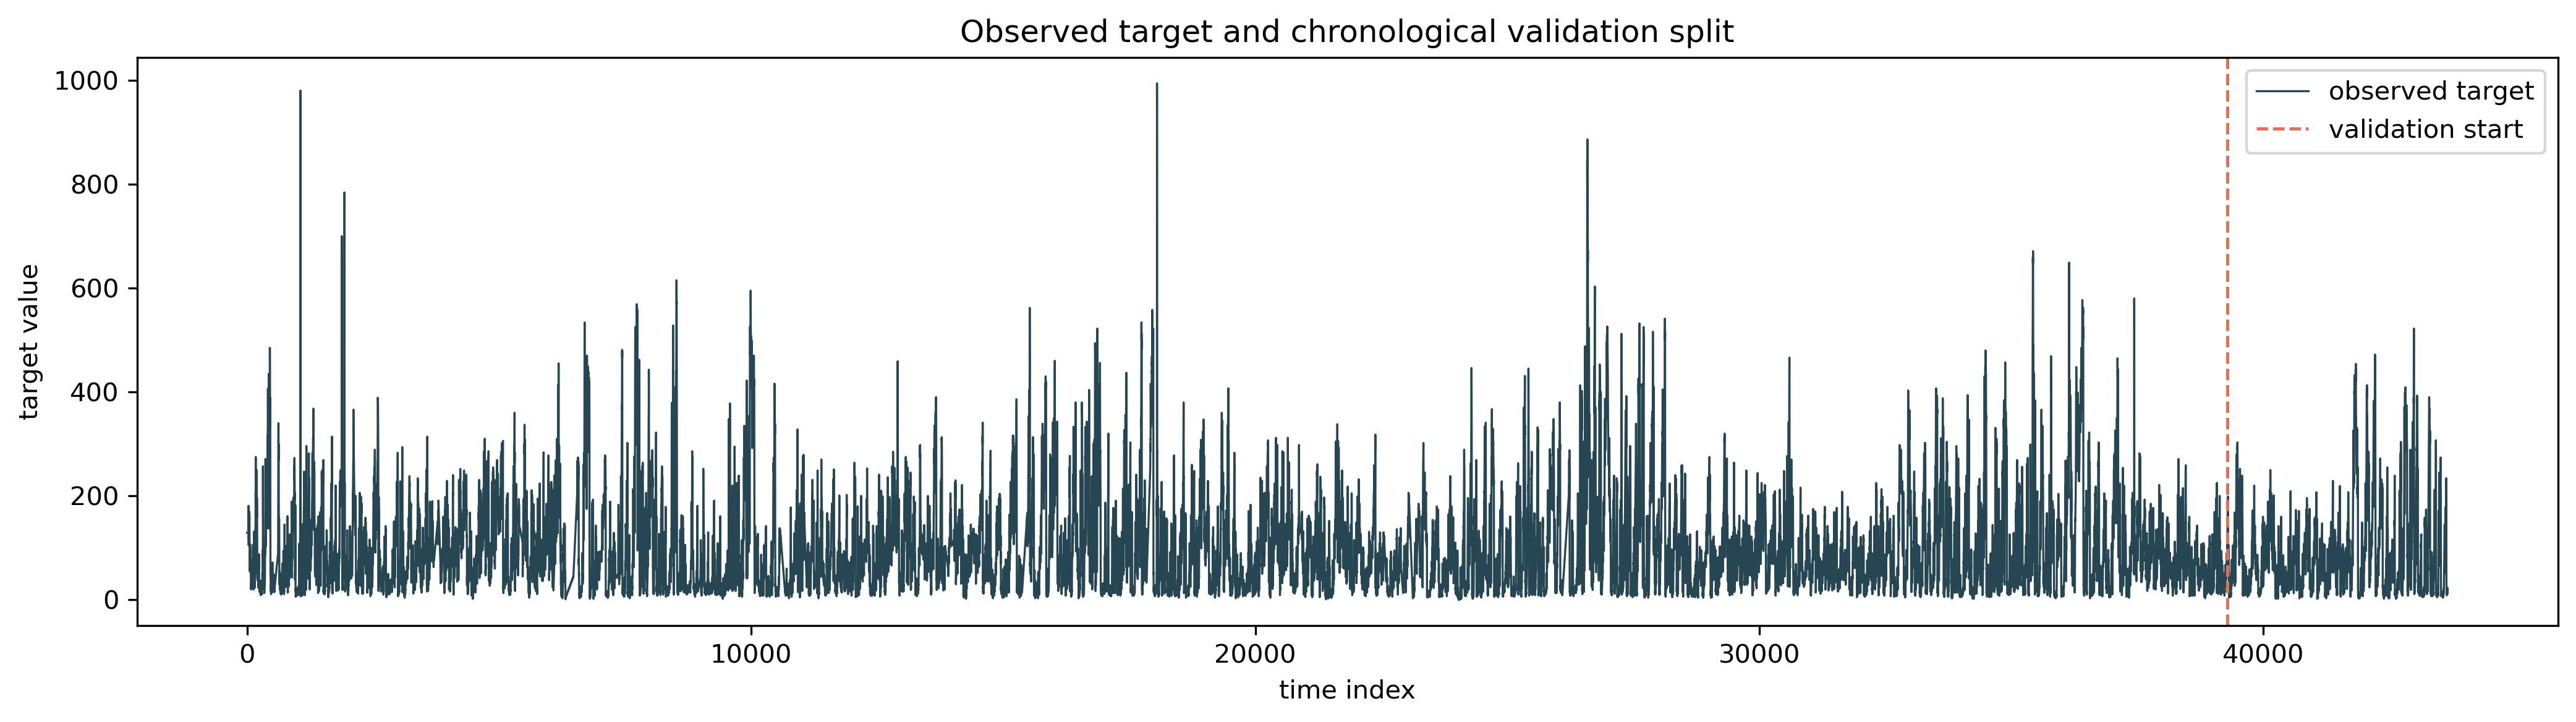
\includegraphics[width=\linewidth]{figures/task2_target_series.png}
\caption{Task 2 observed target series and chronological validation boundary. The large spikes and changing local level motivate block-based validation over the most recent portion of the series.}
\label{fig:t2-series}
\end{figure}

\section{Task 1: Context-Dependent Forecasting}
\label{sec:t1-context}

\subsection{Response 1A: expected and measured ordering}

Before running the comparison, the expected established-station ordering was period-routed ridge, Raw Attention, sensor-specific ridge, then shared ridge. The expectation was that routing by pace would directly handle the changing cycle, Attention would infer useful context-dependent mixing, and station identity would give a smaller improvement over one shared map. For held-out Station 4, the expected ordering was period-routed ridge, Raw Attention, then shared ridge; sensor-specific ridge cannot predict an unseen station.

Table~\ref{tab:t1-part1} revises this ordering using validation measurements. On established Stations 1--3, the measured order is period-routed ridge, Raw Attention, shared ridge, then sensor-specific ridge. Sensor-specific ridge does not improve the shared map because operating pace changes within each station, while splitting the data by station reduces the fitting population. Period routing reduces established-station RMSE from 0.767 for shared ridge to 0.166, a 78.4\pct reduction. Raw Attention reaches 0.434 RMSE without a hand-built router. On held-out Station 4, the predicted order is confirmed: period-routed ridge obtains 0.173 RMSE, Raw Attention obtains 0.624, and shared ridge obtains 0.876.

The product-level values support the same explanation. Period-routed ridge remains between 0.152 and 0.181 RMSE across Products A--C on established stations and between 0.150 and 0.184 on Station 4. Shared ridge is weakest on Product B, with 0.854 established-station RMSE and 0.982 held-out RMSE. Raw Attention is more balanced across products on the established stations, but its held-out errors remain near 0.6 for all three products.

\begin{table}[htbp]
\centering
\caption{Task 1 validation performance for the Part 1 forecasters. MSE is in $(\msq)^2$ and RMSE is in $\msq$. A dash means the model cannot serve the held-out station.}
\label{tab:t1-part1}
\footnotesize
\begin{adjustbox}{max width=\linewidth}
\begin{tabular}{lrrrrrr}
\toprule
Model & Est. MSE & Est. RMSE & Held-out MSE & Held-out RMSE & Parameters & Fit time (s) \\
\midrule
Shared ridge & 0.5878 & 0.7667 & 0.7667 & 0.8756 & 4,608 & 0.015 \\
Sensor-specific ridge & 0.5898 & 0.7680 & -- & -- & 13,824 & 0.057 \\
Period-routed ridge & \textbf{0.0275} & \textbf{0.1659} & \textbf{0.0298} & \textbf{0.1727} & 59,904 & 0.007 \\
Raw Attention & 0.1883 & 0.4339 & 0.3888 & 0.6235 & 368,368 & 67.381 \\
\bottomrule
\end{tabular}
\end{adjustbox}
\end{table}

\subsection{Response 1B: why the rule must depend on context}

One fitted ridge matrix must map every 96-sample context to a 48-sample continuation. For Station 1, the Product A example has period 16.1 samples while the Product C example has period 30.1 samples. Their future peaks require different phase advances. Figure~\ref{fig:t1-contexts} shows the resulting compromise: the fixed shared and sensor-specific maps smooth the oscillation and lose phase or amplitude as the horizon grows. Period routing avoids this compromise by selecting a pace-specific matrix.

Raw Attention uses the same learned projections $W_Q$, $W_K$, and $W_V$ for every example, but the projected queries and keys depend on the current values. Therefore, the matrix
\begin{equation}
  A(x)=\operatorname{softmax}\left(\frac{Q(x)K(x)^\top}{\sqrt{d_h}}\right)
\end{equation}
is recomputed for each context. Figure~\ref{fig:t1-attention} confirms that the Product A and Product C contexts produce different weight maps: the mean absolute weight difference is 0.0116 and the maximum difference is 0.4012. This result shows context-dependent mixing, not recovery of the physical period. The distinction is direct: ridge applies one fixed forecasting operator after fitting, while Attention constructs a new value-mixing operator from every input using shared learned projections.

\begin{figure}[htbp]
\centering
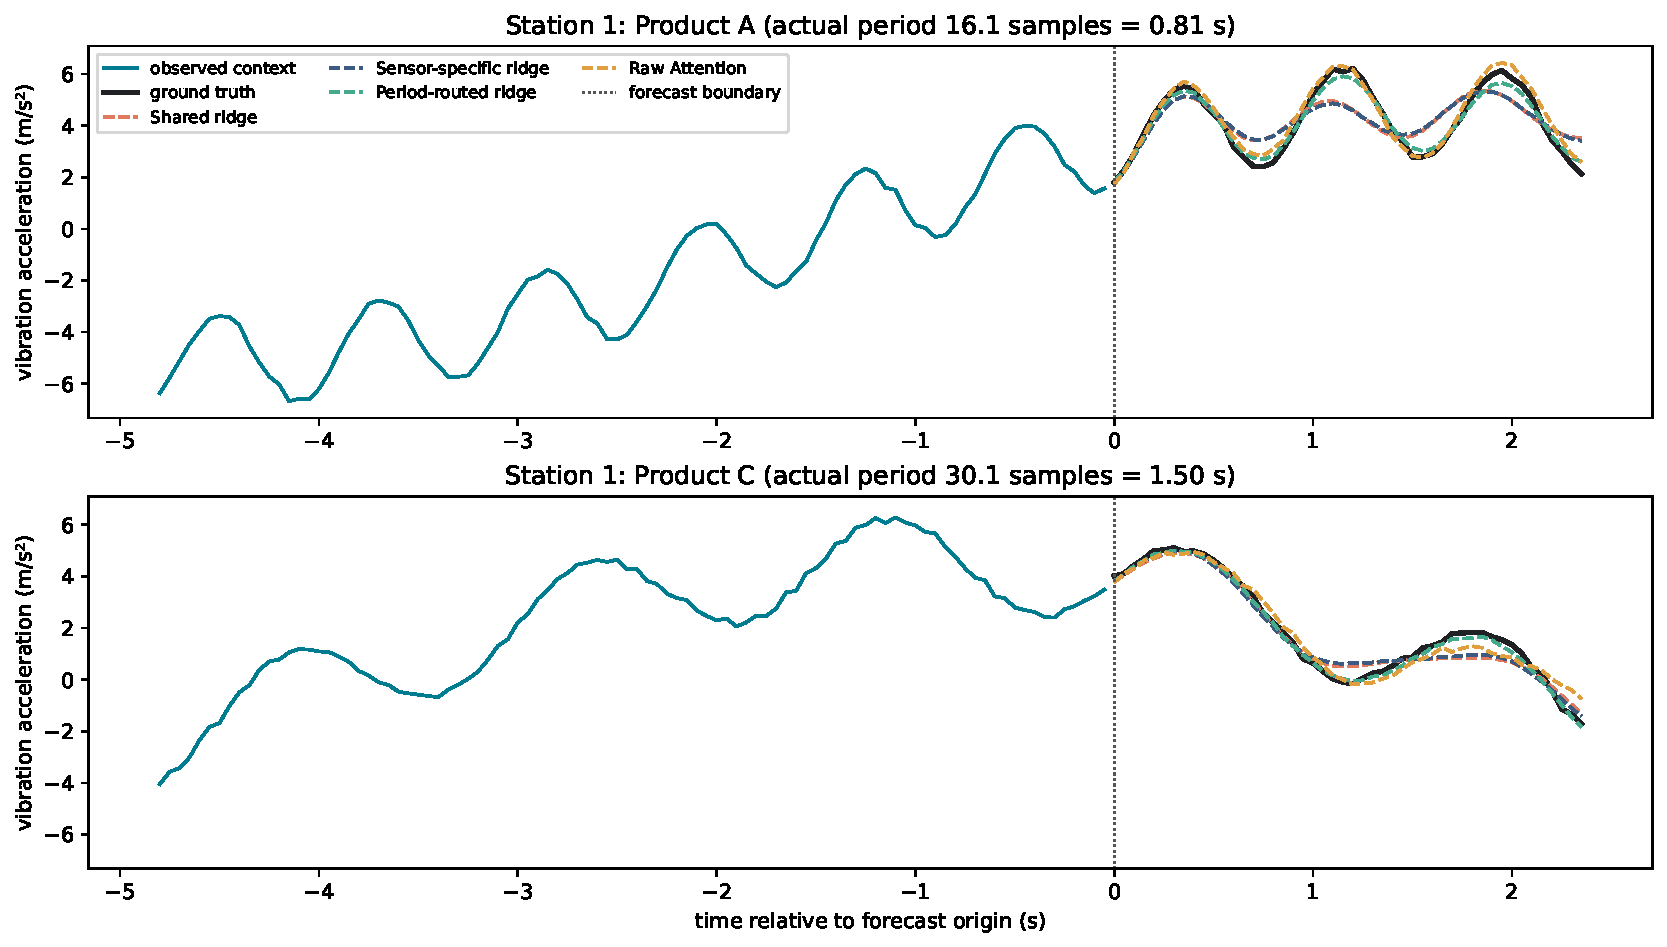
\includegraphics[width=\linewidth]{figures/task1_context_forecasts.pdf}
\caption{Output 1.2: Station 1 forecasts under Product A and Product C. The contexts come from one sensor but require different phase advances because their operating periods differ.}
\label{fig:t1-contexts}
\end{figure}

\begin{figure}[htbp]
\centering
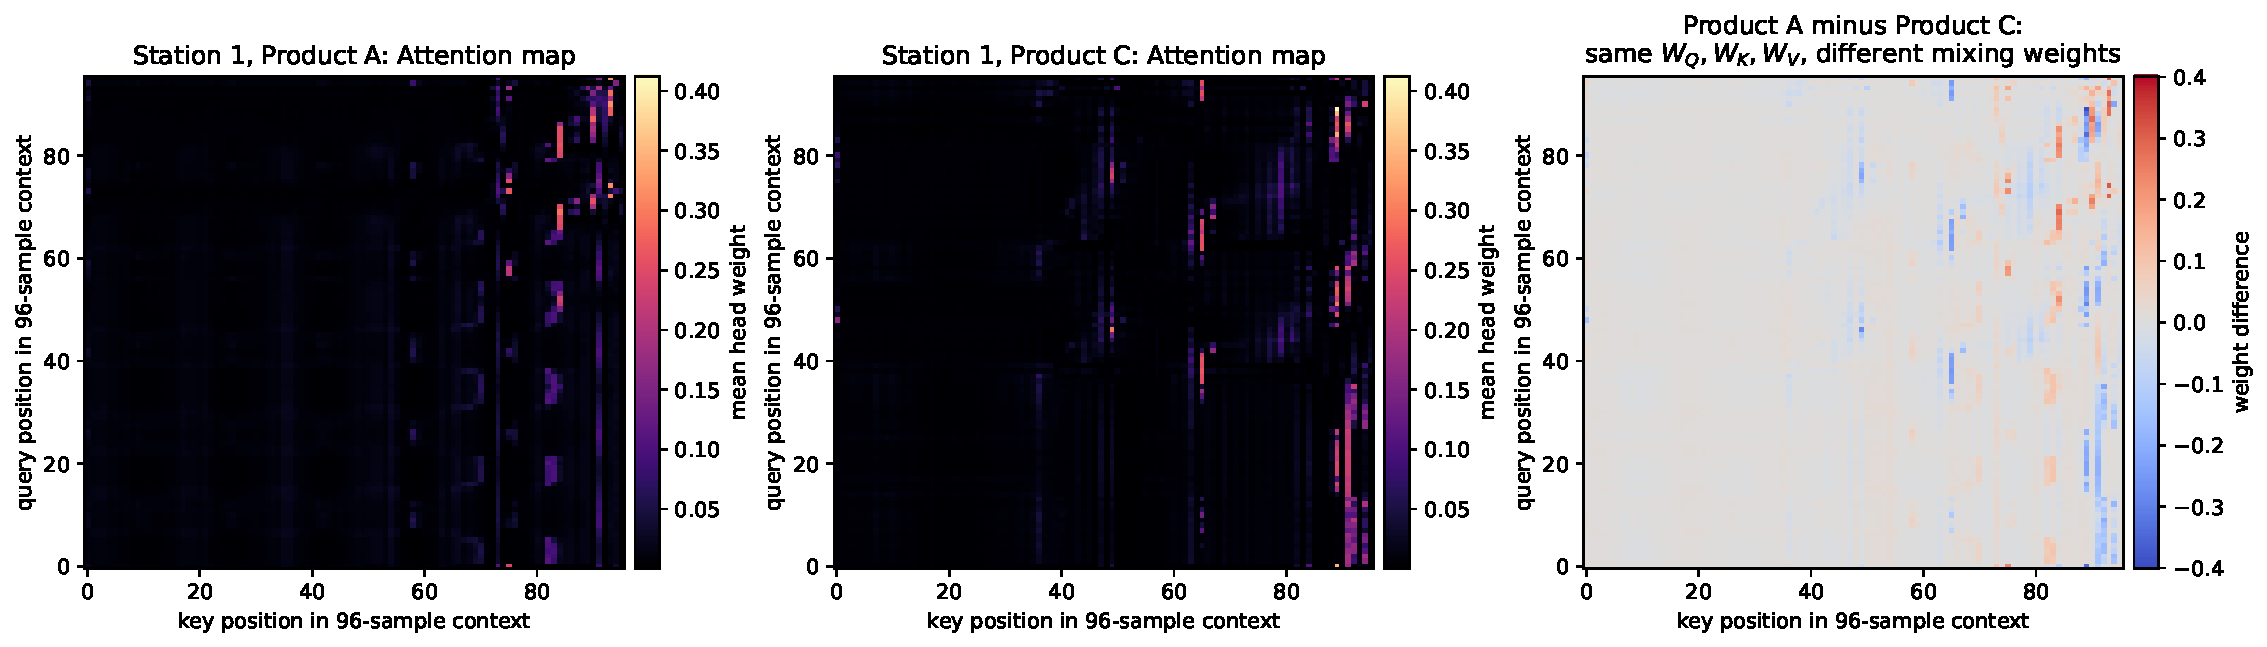
\includegraphics[width=\linewidth]{figures/task1_attention_maps.pdf}
\caption{Output 1.3: mean Attention weights for two contexts and their difference. Shared projections produce different mixing weights because the projected queries and keys depend on the input.}
\label{fig:t1-attention}
\end{figure}

\FloatBarrier

\section{Task 1: Separating Slow Structure from Repetition}
\label{sec:t1-decomposition}

\subsection{Response 2}

The decomposition uses an odd-width centered moving average with endpoint replication. For a context $x$, it computes a smooth component $T$ and remainder $S=x-T$, preserving the exact identity $S+T=x$. Width 41 is selected. As Figure~\ref{fig:t1-decomposition} shows, increasing the width makes the trend smoother and moves more of the oscillation into the remainder. At width 41, the residual preserves the repeating waveform while the trend follows the slow ramp. Endpoint replication keeps the output length fixed, although the repeated boundary values make the edge estimates less symmetric than interior estimates.

The training-only oracle diagnostic compares the period estimated from each residual with the synthetic true period. Raw contexts recover the period within one sample in 68.67\pct of cases. Widths 17, 25, 33, and 41 raise this value to 98.00\pct, 98.92\pct, 99.33\pct, and 99.85\pct, respectively. Width 41 is therefore selected by the primary recovery criterion. Its median absolute period error is 0.216 samples. The oracle is useful here because the true period directly measures whether the filter exposes the known repeating component, and it is used only for design analysis rather than as a model input.

On the validation split, decomposition lowers Attention RMSE from 0.434 to 0.298 on established Stations 1--3 and from 0.624 to 0.449 on held-out Station 4. These are reductions of 31.4\pct and 28.0\pct. The improvement appears across every product. The moving average matches this setting because the baseline varies much more slowly than the vibration. It lets a linear trend head model the smooth component while the encoder focuses on the remainder. This bias would be unsuitable for an abrupt level shift inside the context because the centered average would smear the change across neighboring positions. A change-point-aware piecewise trend would preserve such a jump, but it would assume that the baseline is made of stable segments rather than one smooth curve.

\begin{figure}[htbp]
\centering
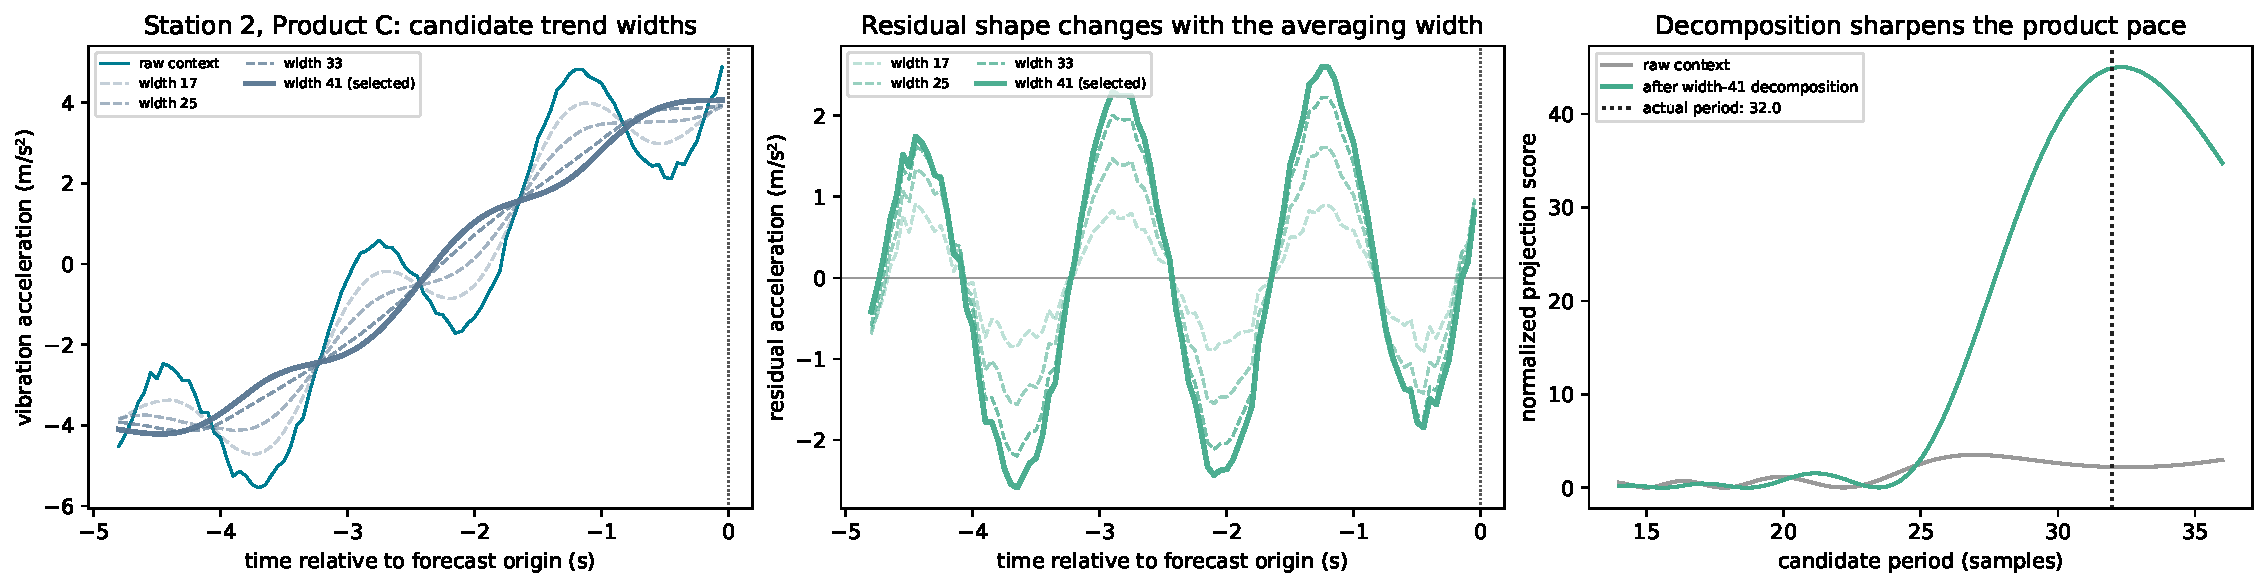
\includegraphics[width=\linewidth]{figures/task1_decomposition_widths.pdf}
\caption{Output 2.1: candidate moving-average trends, their residuals, and the sharper period evidence produced by the selected width 41.}
\label{fig:t1-decomposition}
\end{figure}

\begin{figure}[htbp]
\centering
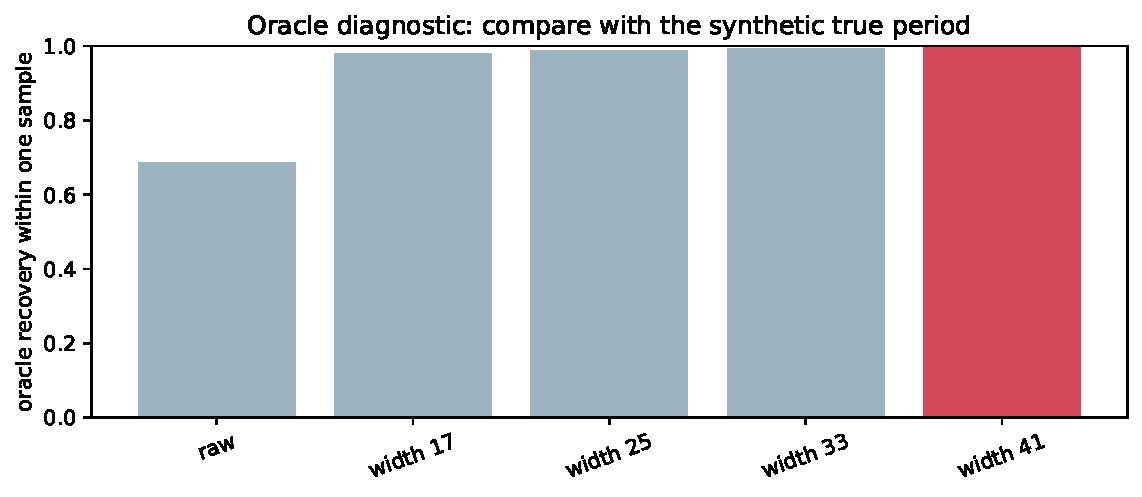
\includegraphics[width=0.72\linewidth]{figures/task1_oracle_recovery.pdf}
\caption{Output 2.2: fraction of synthetic training contexts whose primary period is recovered within one sample.}
\label{fig:t1-oracle}
\end{figure}

\FloatBarrier

\section{Task 1: Mixing by Temporal Delay}
\label{sec:t1-delay}

\subsection{Response 3}

The delay scorer computes one circular correlation value for each displacement. The implementation check on $[1,3,1,3]$ produces scores $[4,-4,4,-4]$, exactly matching direct circular correlation. The aggregation then applies
\begin{equation}
  z_t=\sum_{j=1}^{K}\alpha_j v_{(t-\tau_j)\bmod L}.
\end{equation}
For values $[10,20,30,40]$, delays $[1,3]$, and weights $[0.75,0.25]$, the checked output is $[35,15,25,25]$. In particular, $z_0=35$ confirms that the indexing retrieves earlier values in the required direction. The operation remains differentiable in both the values and normalized weights.

The signal-level diagnostic in Figure~\ref{fig:t1-delay} uses a Product A context with actual period $P=16.13$ samples. Its strongest residual recurrence occurs near lags 16 and 32, which correspond to $P$ and $2P$. The measured correlations are 0.8960 and 0.8969. In the raw context, the large ramp remains similar under many shifts and creates broad correlation that is not specific to the vibration cycle. Removing the slow component produces narrow peaks at repeated displacements. This supports delay mixing because the useful relationships are shared by many pairs with the same displacement.

The diagnostic is computed directly from signal values; it is not a plot of the trained model's query/key scores. Inside the model, delay scores are computed from learned projected features. Delay mixing would be a poor assumption for an isolated transient. Repeating a selected displacement would copy the event to positions where no related event exists, while ordinary Attention could connect the transient to a specific position without assuming global recurrence.

\begin{figure}[htbp]
\centering
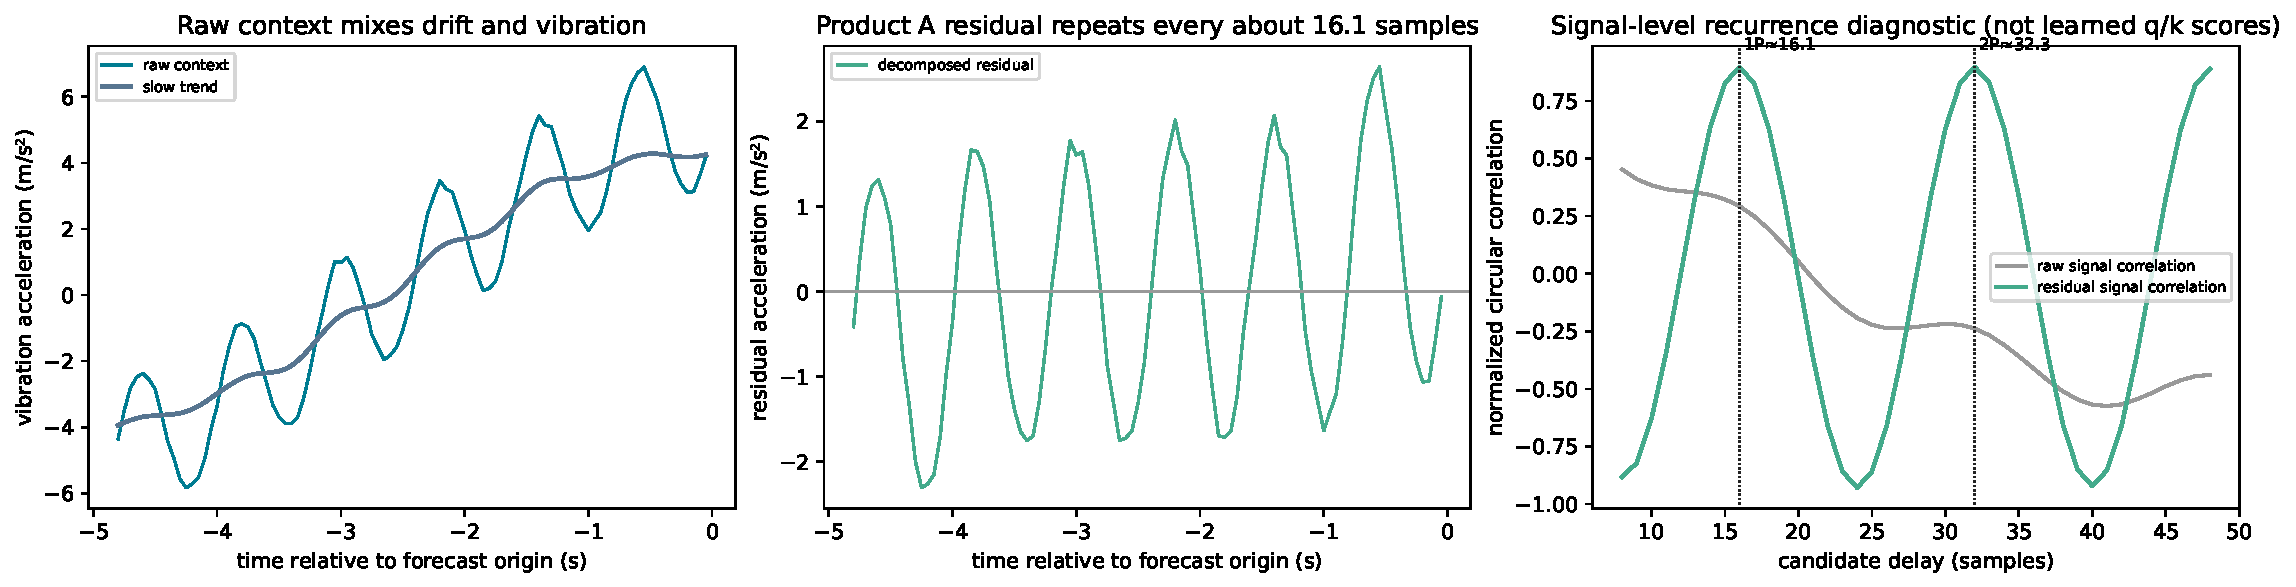
\includegraphics[width=\linewidth]{figures/task1_delay_recurrence.pdf}
\caption{Output 3.2: raw drift-plus-vibration context, decomposed remainder, and signal-level circular correlation. Peaks near 16 and 32 samples match one and two periods.}
\label{fig:t1-delay}
\end{figure}

\FloatBarrier

\section{Task 1: Design Comparison and Deployment}
\label{sec:t1-deploy}

\subsection{Response 4}

Before Output 4.1, I expected decomposition to help most when the slow component was prominent because it gives the ramp a separate trend path and leaves the mixer a cleaner repeating signal. I expected both upgrades to help, with partly overlapping gains because both address the same drift-plus-repetition structure.

On established-station validation, decomposition lowers Attention MSE from 0.1883 to 0.0887, while delay mixing lowers the raw model to 0.0469. With decomposition already active, delay mixing reaches 0.0310; with delay mixing active, decomposition improves MSE from 0.0469 to 0.0310. Thus, both switches help in both settings, but the combined gain is smaller than the sum of their separate gains. Errors generally rise with horizon, especially for Raw Attention and on held-out Station 4 (Figure~\ref{fig:t1-horizon}). The Autoformer-inspired model is the best neural design, with RMSE 0.1760 on established stations and 0.2182 on Station 4. Period-routed ridge is selected for both deployments because it is still more accurate, fits in 0.007 seconds, and uses 59,904 parameters. Its validation RMSEs are 0.1659 and 0.1727, and its final-test RMSEs are 0.1611 and 0.1826 for established and held-out populations, respectively.

\begin{table}[htbp]
\centering
\caption{Task 1 validation comparison used for deployment. MSE is in $(\msq)^2$ and RMSE is in $\msq$.}
\label{tab:t1-all}
\footnotesize
\begin{adjustbox}{max width=\linewidth}
\begin{tabular}{lrrrrrr}
\toprule
Model & Est. MSE & Est. RMSE & Held-out MSE & Held-out RMSE & Parameters & Fit time (s) \\
\midrule
Shared ridge & 0.5878 & 0.7667 & 0.7667 & 0.8756 & 4,608 & 0.015 \\
Sensor-specific ridge & 0.5898 & 0.7680 & -- & -- & 13,824 & 0.057 \\
Period-routed ridge & \textbf{0.0275} & \textbf{0.1659} & \textbf{0.0298} & \textbf{0.1727} & 59,904 & 0.007 \\
Raw Attention & 0.1883 & 0.4339 & 0.3888 & 0.6235 & 368,368 & 67.381 \\
Raw delay mixer & 0.0469 & 0.2165 & 0.1091 & 0.3303 & 368,370 & 93.747 \\
Attention + decomposition & 0.0887 & 0.2977 & 0.2016 & 0.4490 & 373,024 & 136.215 \\
Autoformer-inspired & 0.0310 & 0.1760 & 0.0476 & 0.2182 & 373,026 & 197.650 \\
\bottomrule
\end{tabular}
\end{adjustbox}
\end{table}

\begin{figure}[htbp]
\centering
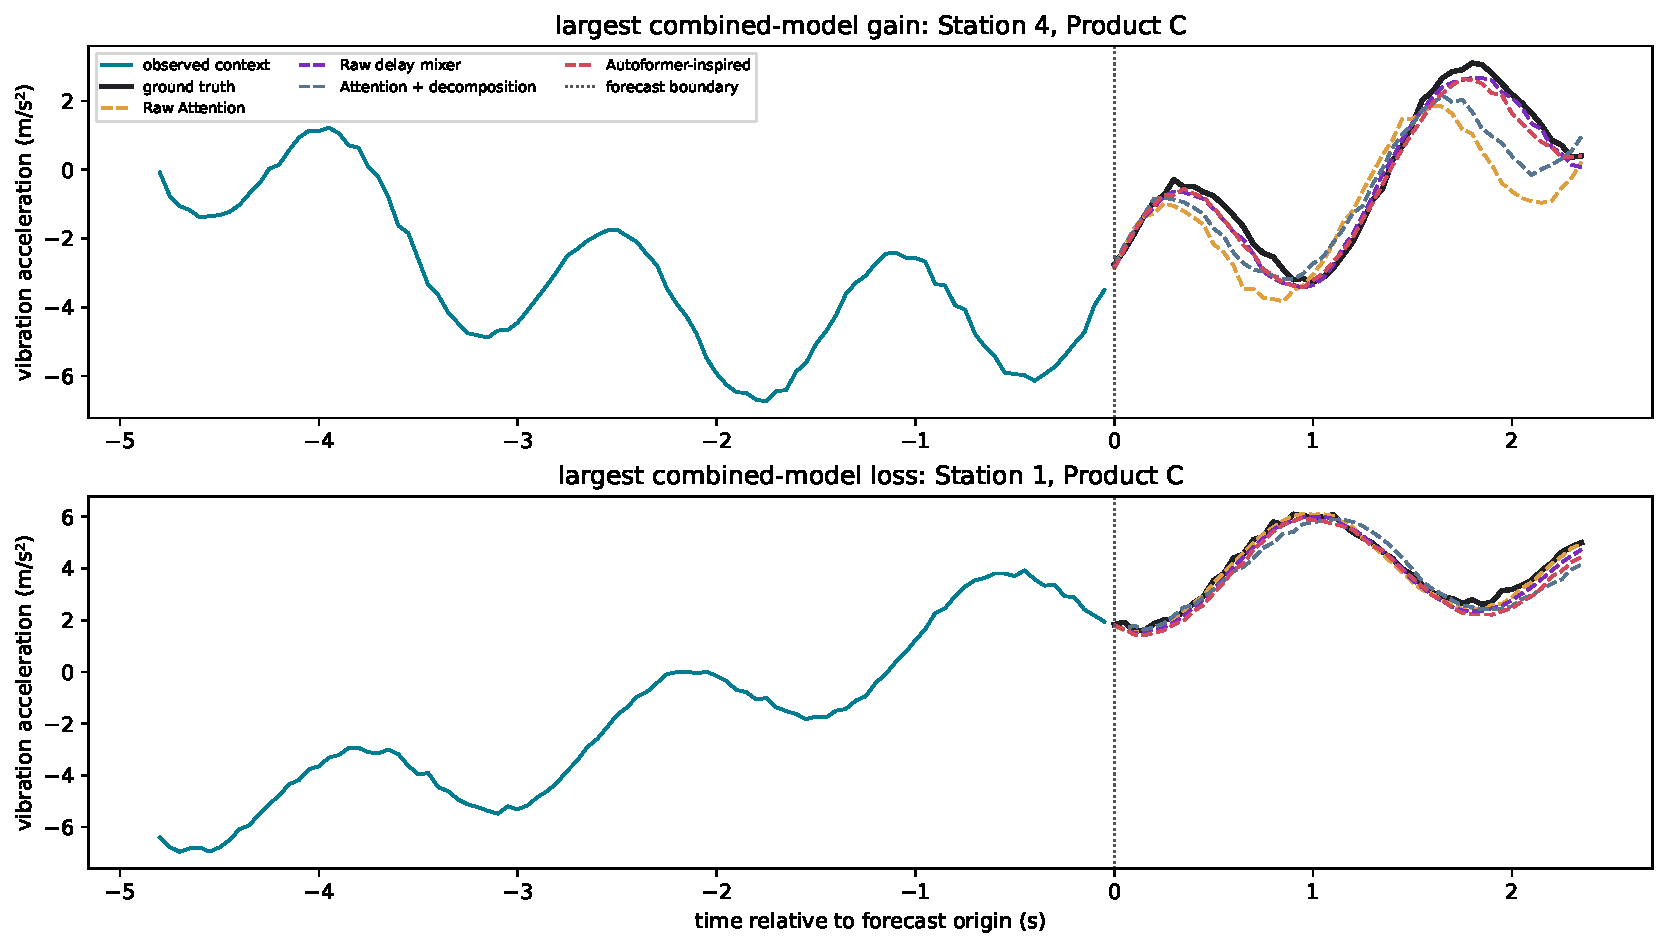
\includegraphics[width=\linewidth]{figures/task1_combined_cases.pdf}
\caption{Output 4.1 forecast cases with the largest gain and loss for the combined neural model. The aggregate table, rather than one selected case, determines deployment.}
\label{fig:t1-combined}
\end{figure}

\begin{figure}[htbp]
\centering
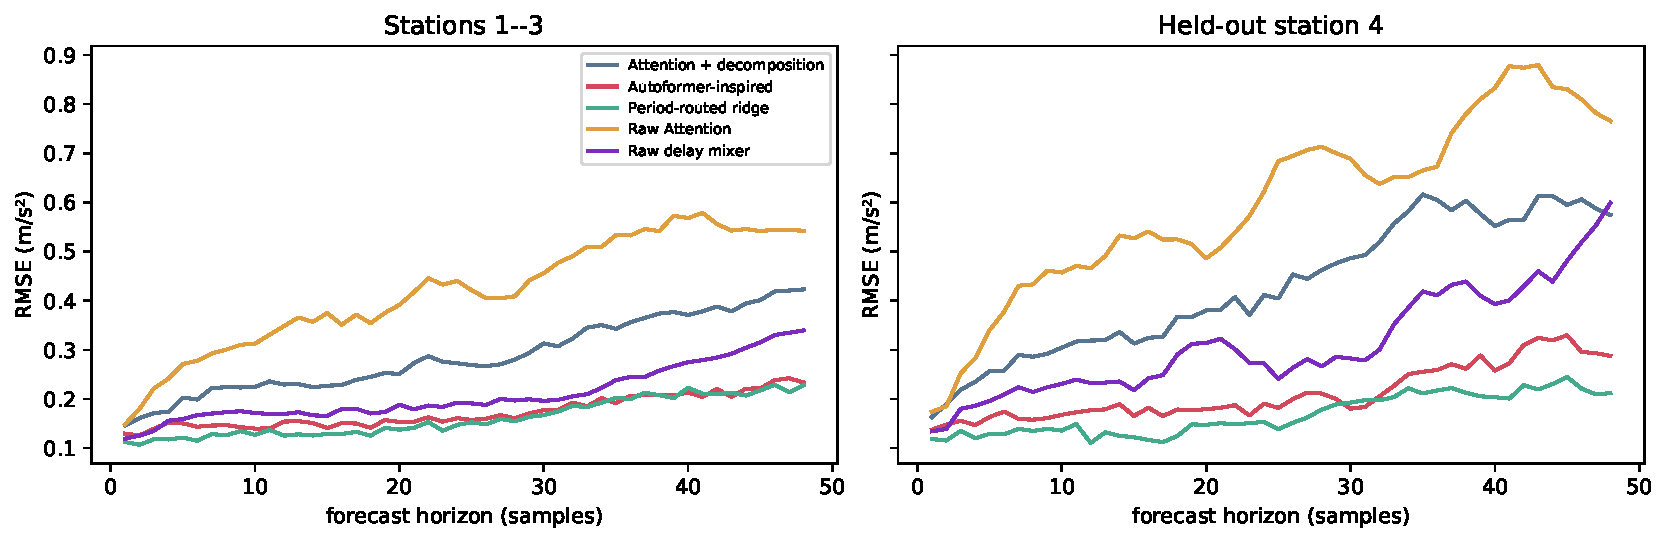
\includegraphics[width=\linewidth]{figures/task1_horizon_error.pdf}
\caption{Output 4.2: physical-unit RMSE by forecast step for established Stations 1--3 and held-out Station 4.}
\label{fig:t1-horizon}
\end{figure}

\FloatBarrier

\section{Task 2: Autoformer Forecasting}
\label{sec:t2}

\subsection{Model design}

The Task 2 model is a from-scratch encoder-decoder Autoformer based on \citet{wu2021autoformer}. The initial moving average splits the input into seasonal and trend streams. Progressive decomposition is repeated after the auto-correlation and feed-forward sublayers, so each following block receives a seasonal remainder. The decoder adds the extracted trend contributions to a trend initialization and adds its seasonal projection at the output.

Auto-correlation projects the hidden sequence into queries, keys, and values, computes correlation for all delays using the real FFT, selects $k=\lfloor 2\log L\rfloor$ delays, and aggregates shifted values using softmax weights. Training uses delays selected from the batch-mean scores, while inference selects delays per example. The encoder has two layers and the decoder has one layer. Model width is 32, with four heads and feed-forward width 128. Dropout is 0.1 and the activation is GELU.

External variables enter through a learned linear projection that is added to the target-value embedding. Historical external values are supplied to the encoder. The decoder receives the final 168 historical external rows followed by the 168 known future rows. This placement makes future external information available directly at each forecast position. A smoke test verifies finite outputs, expected shape, exact seasonal-plus-trend reconstruction, and gradient flow. A 200-step one-batch test reduces training-mode MSE by 90.81\pct, confirming that the implementation can fit a small sample.

\begin{table}[htbp]
\centering
\caption{Final Task 2 Autoformer configuration.}
\label{tab:t2-config}
\footnotesize
\begin{tabular}{lc@{\qquad}lc}
\toprule
Setting & Value & Setting & Value \\
\midrule
Input / label / prediction length & 672 / 168 / 168 & Model / feed-forward width & 32 / 128 \\
Encoder / decoder layers & 2 / 1 & Attention heads & 4 \\
Delay factor & 2.0 & Moving-average width & 13 \\
External variables & 10 & Dropout & 0.1 \\
Batch size & 64 & Learning rate & $10^{-3}$ \\
Final epochs & 3 & Trainable parameters & 42,561 \\
\bottomrule
\end{tabular}
\end{table}

\subsection{Moving-average width ablation}

Widths 13, 25, and 49 are compared with all ten external variables and matched seeds 0 and 1. All other settings are fixed. Table~\ref{tab:t2-width} shows that width 13 has the lowest mean validation RMSE, MAE, and scaled MSE. It also has the smallest RMSE standard deviation. Width 25 has lower training error but worse validation error, while width 49 is worse on every validation metric. The result selects width 13 because model choice is based on chronological validation performance rather than training fit.

Figure~\ref{fig:t2-width} illustrates one validation block using the best run for each width. All three forecasts capture some broad changes, but their timing and baseline differ. The table aggregates all 26 validation blocks and both seeds, so it provides the selection evidence. Relative to widths 25 and 49, width 13 lowers mean validation RMSE by 3.7\pct and 10.0\pct.

\begin{table}[htbp]
\centering
\caption{Task 2 moving-average-width ablation with external variables. Values are mean $\pm$ standard deviation across seeds 0 and 1. MSE is computed in standardized target space; RMSE and MAE are in the original target scale.}
\label{tab:t2-width}
\footnotesize
\begin{tabular}{lcccc}
\toprule
Width & Validation MSE & Validation RMSE & Validation MAE & Validation sMAPE \\
\midrule
13 & \textbf{0.4744 $\pm$ 0.0059} & \textbf{62.02 $\pm$ 0.59} & \textbf{44.84} & \textbf{66.00\pct} \\
25 & 0.5145 $\pm$ 0.0243 & 64.42 $\pm$ 1.91 & 47.30 & 69.91\pct \\
49 & 0.5768 $\pm$ 0.0436 & 68.88 $\pm$ 2.92 & 51.82 & 69.30\pct \\
\bottomrule
\end{tabular}
\end{table}

\begin{figure}[htbp]
\centering
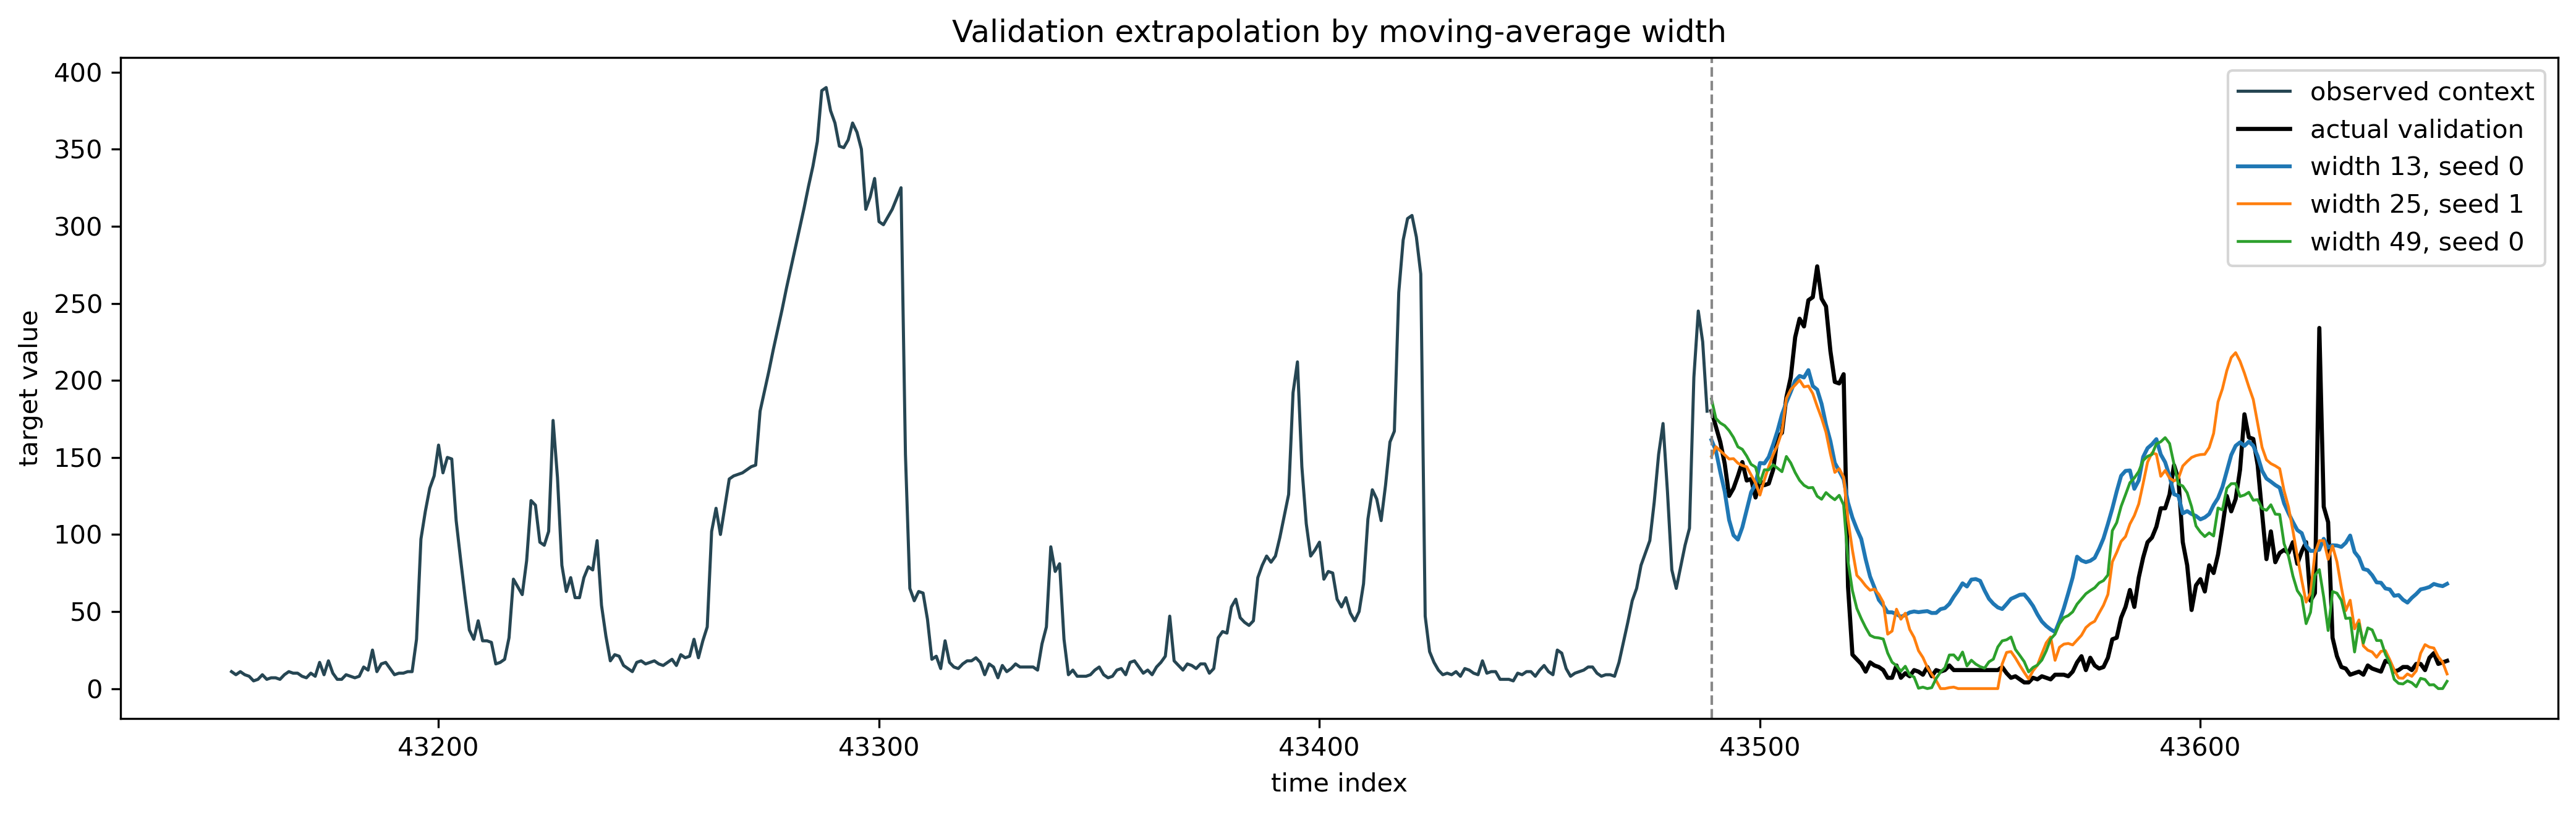
\includegraphics[width=\linewidth]{figures/task2_width_comparison.png}
\caption{Representative validation forecasts for moving-average widths 13, 25, and 49. The aggregate multi-block results in Table~\ref{tab:t2-width} select width 13.}
\label{fig:t2-width}
\end{figure}

\subsection{External-data ablation}

The selected width 13 is evaluated with and without all external variables using matched seeds 0, 1, and 2. The external-data model wins on validation RMSE for all three seeds. It reduces mean RMSE from 88.31 to 62.19, mean MAE from 66.44 to 45.58, and mean sMAPE from 78.42\pct to 65.64\pct. The RMSE reduction is 29.6\pct. The improvement is much larger than the across-seed standard deviations, giving a clear selection decision.

The comparison in Figure~\ref{fig:t2-external} explains the numerical gap. The target-only forecast remains close to one level through most of the horizon, while the external-data model follows several broad rises and falls. This result shows that the ten external variables collectively contain useful information about future target movement. The experiment evaluates the complete group, so it does not assign the improvement to one individual variable.

\begin{table}[htbp]
\centering
\caption{Task 2 external-data ablation at width 13. Values are mean $\pm$ standard deviation across three matched seeds.}
\label{tab:t2-external}
\footnotesize
\begin{tabular}{lccccc}
\toprule
Inputs & Validation MSE & Validation RMSE & Validation MAE & sMAPE & Parameters \\
\midrule
Target only & 0.9389 $\pm$ 0.0029 & 88.31 $\pm$ 0.14 & 66.44 $\pm$ 0.08 & 78.42 $\pm$ 0.20\pct & 41,921 \\
Target + external & \textbf{0.4754 $\pm$ 0.0045} & \textbf{62.19 $\pm$ 0.51} & \textbf{45.58 $\pm$ 1.30} & \textbf{65.64 $\pm$ 1.00\pct} & 42,561 \\
\bottomrule
\end{tabular}
\end{table}

\begin{figure}[htbp]
\centering
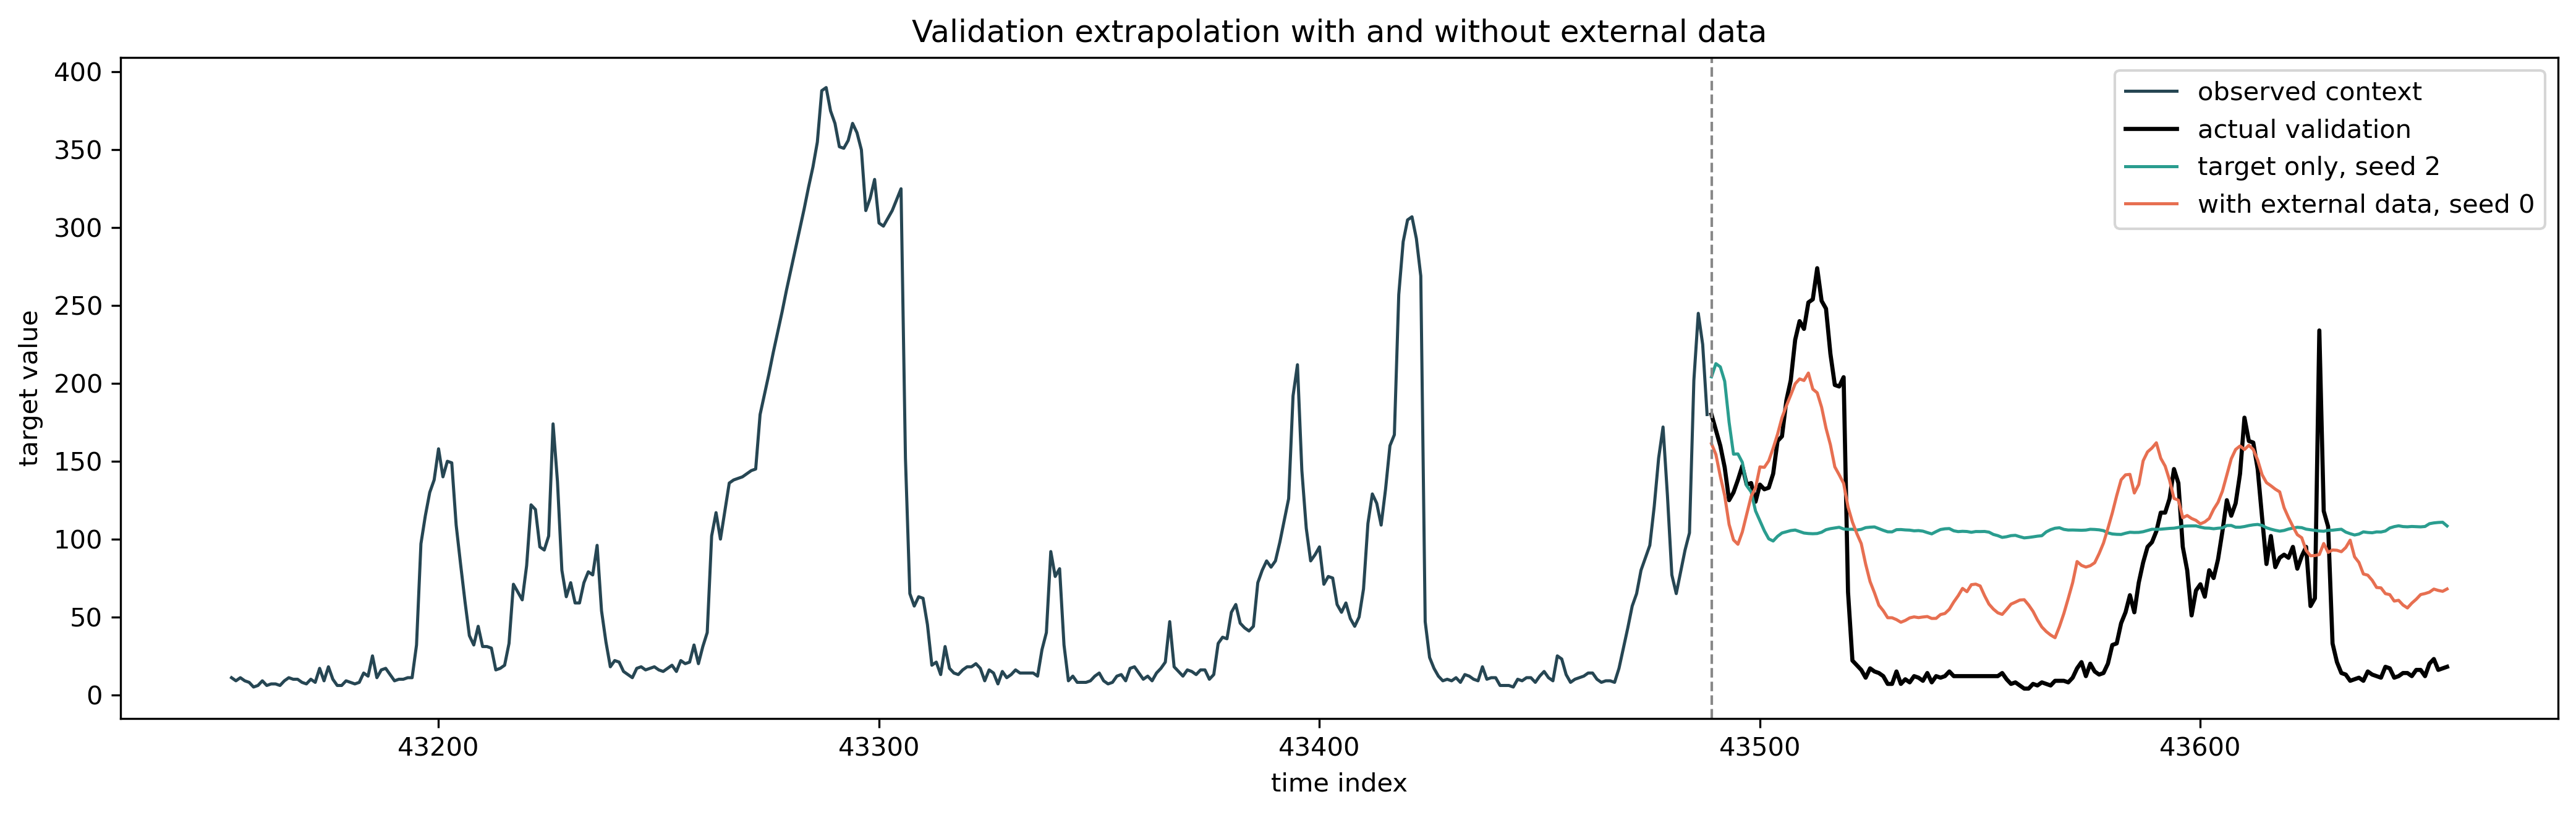
\includegraphics[width=\linewidth]{figures/task2_external_comparison.png}
\caption{Representative validation forecasts with and without external variables. The external-data model follows major changes that the target-only model misses.}
\label{fig:t2-external}
\end{figure}

\subsection{Final training and forecast}

The final model uses width 13 and all ten external variables. It is trained from seed 0 on every observed target value for three epochs. Physical-unit training RMSE decreases from 73.03 to 68.28 and then 65.57. The resulting model contains 42,561 trainable parameters and produces exactly 168 finite values for indices 43,657 through 43,824.

Figure~\ref{fig:t2-final} shows the last 336 observed values and the final forecast. The prediction begins near the recent level, rises to a broad peak near 180, represents several additional cycles, and then falls toward zero at the end. The zero-valued tail follows the stated non-negativity rule after inverse scaling. The hidden target values are not available locally, so they are evaluated only through the public leaderboard.

\begin{figure}[htbp]
\centering
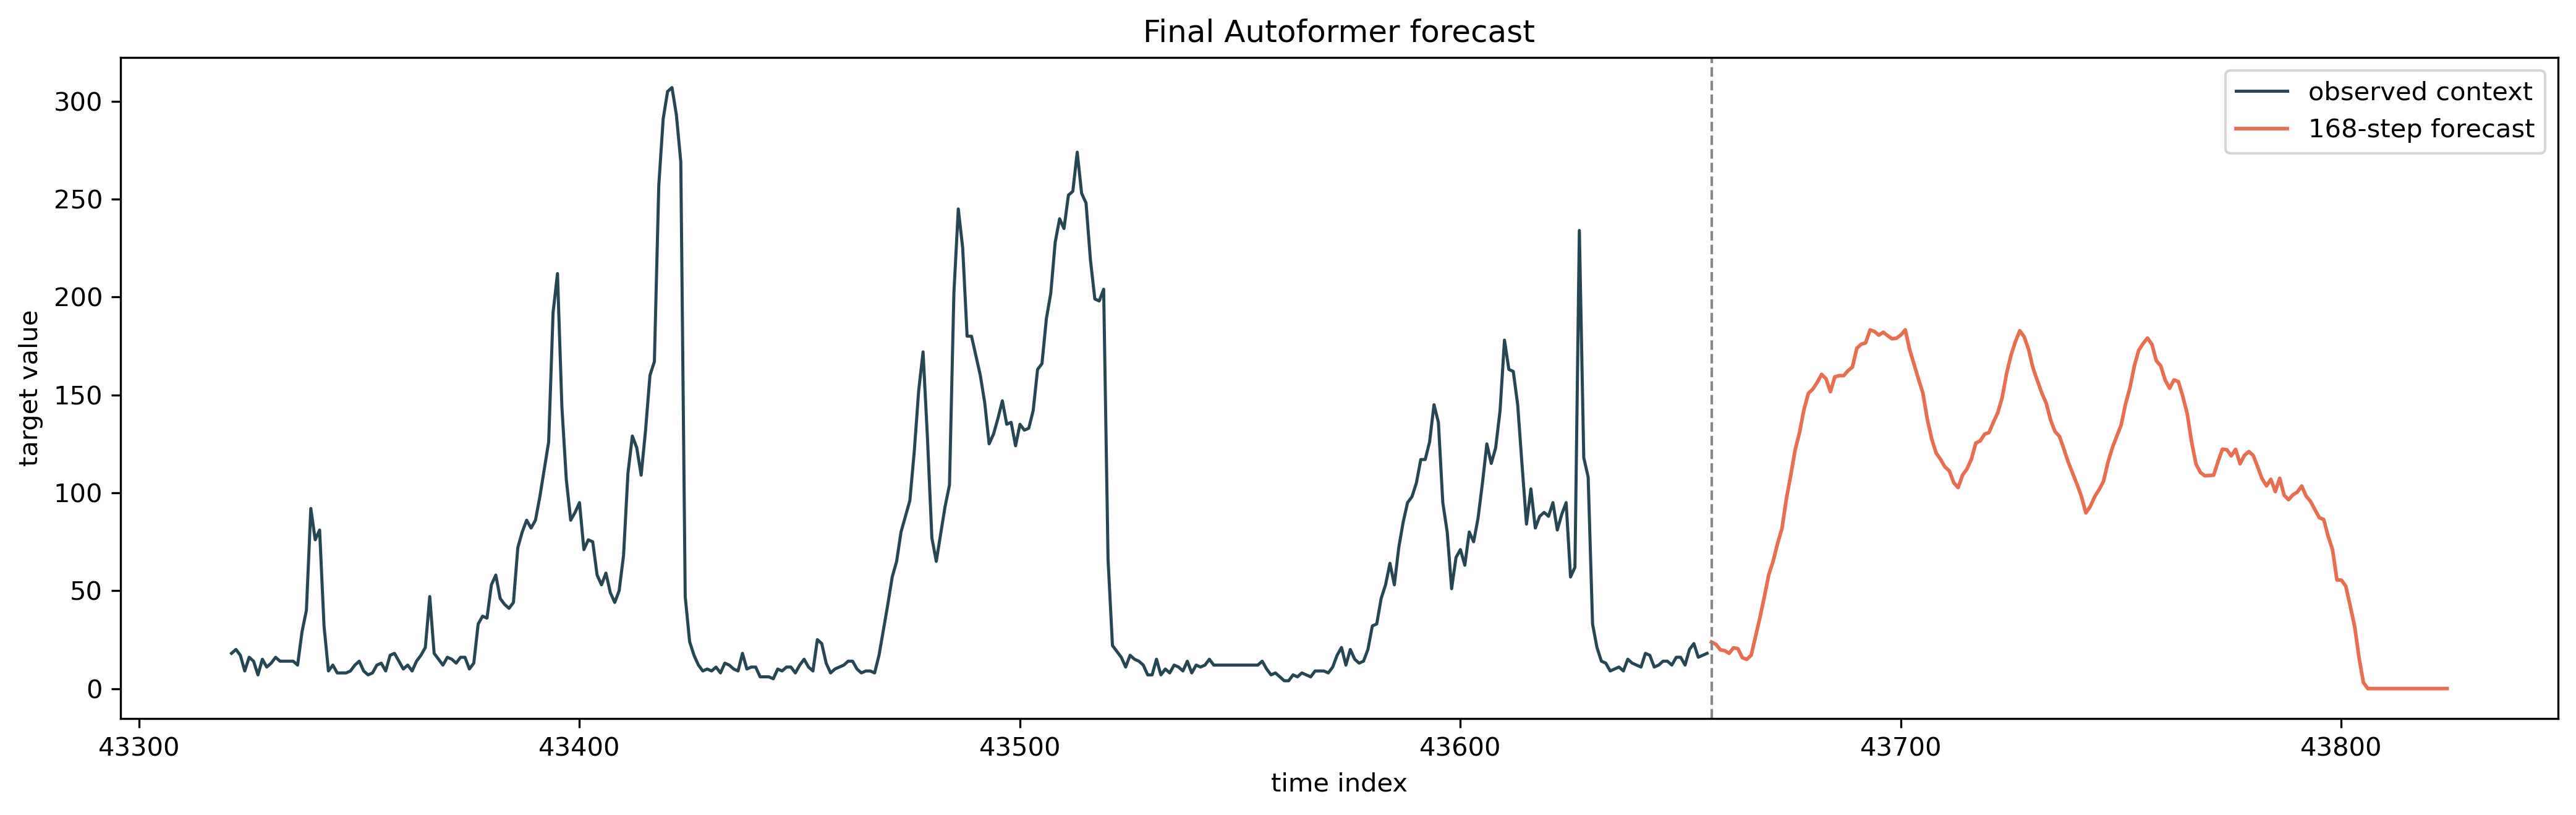
\includegraphics[width=\linewidth]{figures/task2_final_forecast.png}
\caption{Final 168-step Autoformer forecast after refitting the selected configuration on all observed values.}
\label{fig:t2-final}
\end{figure}

\subsection{Hidden-test leaderboard result}

The final forecast obtains MAE 62.3154, RMSE 84.5748, and sMAPE 75.99\pct on the 168-step hidden continuation. With 42,561 trainable parameters and three declared training epochs, its leaderboard score is 84.5764. These values are reported as final hidden-test evaluation only. Width 13, external-data use, and every other model choice were selected from the chronological validation experiments before this result was observed.

\begin{table}[htbp]
\centering
\caption{Final Task 2 result on the public hidden-test leaderboard.}
\label{tab:t2-leaderboard}
\footnotesize
\begin{tabular}{rrrrrr}
\toprule
MAE & RMSE & sMAPE & Parameters & Epochs & Score \\
\midrule
62.3154 & 84.5748 & 75.99\pct & 42,561 & 3 & 84.5764 \\
\bottomrule
\end{tabular}
\end{table}

\FloatBarrier

\section{Discussion}
\label{sec:discussion}

The two tasks give a consistent view of temporal inductive bias. In Task 1, Raw Attention improves over fixed shared and sensor-specific mappings because it changes its mixing weights with the context. Decomposition improves the representation by separating a slow ramp, and delay mixing gives the larger individual neural gain because the simulated vibration is organized directly by repeated displacement. Their combination gives the best neural result. However, period-routed ridge remains better because the data generator makes operating pace the correct routing variable and the supplied estimator exposes it directly. The simplest model wins when its assumption closely matches the process.

Task 2 does not contain one stable cycle that can be routed by a hand-built period estimate. The full Autoformer is useful because it can discover several delays while repeatedly separating local trend and seasonal structure. Width 13 performs best on the chronological validation region, showing that the moving-average scale must be selected from evidence rather than transferred from Task 1. The external-data result is equally important: model architecture alone cannot replace useful information. Supplying known future factors gives the decoder signals that the target history does not contain, reducing RMSE for every tested seed.

The validation protocols reflect the two settings. Task 1 has named established and held-out sensor populations and reports physical-unit results separately. Task 2 has one long series, so recent chronological blocks provide the closest available estimate of future performance. In both cases, selection is made on validation data and final evaluation is kept separate.

\section{Limitations}
\label{sec:limitations}

Task 1 is synthetic and its strongest baseline uses a reliable estimate of the known generating period. That result demonstrates the value of a correct physical variable, but it does not imply that period routing will dominate on a less regular series. The neural comparison also uses one model seed, so small differences should not be treated as general rankings. The large gaps between Raw Attention, the delay mixer, and the combined model are the main evidence.

Task 2 uses three seeds for the external-data decision but only two seeds for width selection. Architectural exploration is also limited. The study keeps one compact Autoformer design and mainly varies decomposition width and external-data use; it does not systematically search model width, encoder-decoder depth, head count, input length, delay factor, covariate-fusion strategy, or alternative decomposition operators. This restricted search may partly explain why hidden-test RMSE is higher than chronological validation RMSE. The external ablation also tests all ten variables as one group. It establishes that the group is useful, while leaving individual feature importance unresolved.

\section{Conclusion}

Task 1 shows that context-dependent mixing is better than one fixed mapping when operating pace changes. Moving-average decomposition and delay mixing both improve neural forecasts, and their combination is the strongest neural design. Period-routed ridge is still selected for deployment because its hand-built assumption matches the controlled data and gives the best validation accuracy at low fitting cost. Task 2 shows how the same structural ideas extend to a real anonymized series through a full Autoformer. Chronological experiments select width 13 and show a consistent benefit from external variables across three seeds. The final model uses 42,561 parameters, three training epochs, and obtains 84.5748 RMSE on the required 168-step hidden forecast. Across both tasks, the main result is direct: a useful temporal structure improves forecasting when it matches the signal, and informative inputs remain as important as model design.

\begin{thebibliography}{1}

\bibitem[Wu et~al.(2021)Wu, Xu, Wang, and Long]{wu2021autoformer}
Haixu Wu, Jiehui Xu, Jianmin Wang, and Mingsheng Long.
\newblock Autoformer: Decomposition transformers with auto-correlation for long-term series forecasting.
\newblock In \emph{Advances in Neural Information Processing Systems}, volume 34, pages 22419--22430, 2021.

\end{thebibliography}

\end{document}
